\documentclass{standalone}
\usepackage{tikz}
\usetikzlibrary{hobby}
\begin{document}
\newcommand\helpgrid[3]{ % args: x1 y1, step. The grid starts from (0,0) to (x1,y1) with given step
    \draw[help lines, color=gray, dashed] (0,0) grid[step={(#3,#3)}] (#1,#2);
    \foreach \x in {0,1,...,#1}
        {
            \node at (\x,0) {\textbf{\x}};
        }
    \foreach \y in {0,1,...,#2}
        {
            \node at (0,\y) {\textbf{\y}};
        }
}
\newcommand{\protein}{\path[draw,use Hobby shortcut,closed=true,fill=blue!20](3, 2) .. (2, 4) .. (4, 5) .. (4, 4) .. (5, 4);}
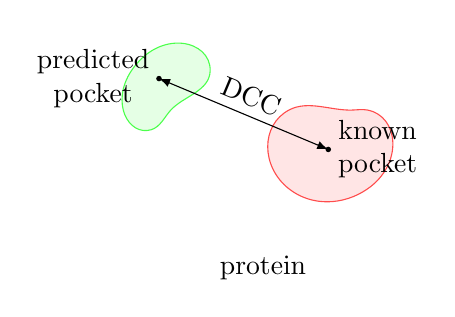
\begin{tikzpicture}
    % \helpgrid{8}{8}{0.5}
    % \path[draw,use Hobby shortcut,closed=true,fill=blue!20]
    %     (3, 2) .. (2, 4) .. (4, 5) .. (4, 4) .. (5, 4);
    \protein
    \path[draw,color=red!70,use Hobby shortcut,closed=true,fill=red!20,fill opacity=0.5]
        (4, 4) .. (4, 5) .. (4.8, 5) .. (5, 5) .. (5, 4);
    \coordinate (center1) at (4.5, 4.5);
    \fill (center1) circle (1pt);
    \node[anchor=west, align=center] at (center1) {known\\pocket};
    \path[draw, color=green!70, use Hobby shortcut,closed=true,fill=green!20,fill opacity=0.5]
        (2.25, 4.75) .. (2.5, 5) .. (3, 5.5) .. (2, 5.5);
    \coordinate (center2) at (2.35, 5.4);
    \fill (center2) circle (1pt);
    \node[anchor=east, align=center] at (center2) {predicted\\pocket};
    \path[draw, latex-latex] (center1) -- node[above, sloped] {DCC} (center2);
    \node[anchor=west] at (3, 3) {protein};
\end{tikzpicture}
\end{document}
